When simulating physical phenomena one must choose a model which fits
the phenomena being modeled. The level set method (LSM), is a method
for modelling phenomena that can be described in terms of moving level
sets.
%
A level set in itself is only a mathematical function that groups
variables which have the same function value. It describes a
parametric function in one dimension higher than its original domain,
gaining the ability to describe more than one not colocated level set
in the same structure.
%
A two dimensional level set is known as a level curve or isocontour,
which uses two dimensions to describe curves. We encounter isocontours
in everyday life as pressure information in the weather forecast and
terrain elevation on maps.
%
A three dimensional level set is
known as a level surface or isosurface, and is used, as suggested be
it's name, to describe surfaces.  A general a level set in n
dimensions is used to describe n-1 dimensional objects. Mathematically
a level set is define as follows:

\begin{equation}
\{ (x_1,...,x_n) \} | f(x_1,...,x_n) = c
\end{equation}

In words this means that all values of $v_i$ leading to a function
value of $c$ defines the level set $c$.
%
The level set in its own right does not make a simulation. Unless it
is evolved over times it stays the same. To evolve the level set over
time, partial differential equations (PDEs) describing the physical
phenomena needs to be solved to move the level sets.
%
Typical phenomena modeled by the LSM includes: computational fluid
dynamics (CFG), and fire and explosion simulation. 

In this report, we will explain what the level set method is and what
its applications are. Furthermore, we will provide code examples of
how to implement the mathematical formulas.

In figure \vref{fig:heightmap} we see two figures describing a two dimensional and
three dimensional view of an island. Figure \vref{fig:isocontour-2d} describes an
isocontour map of heights where the color indicates the height of each
point. The brighter the color the higher the point. Figure
\vref{fig:isocontour-3d} shows the corresponding 3d view.

\begin{figure}[h]
\begin{center}
  \subfloat[Two dimensional view of an isocontour map]{
    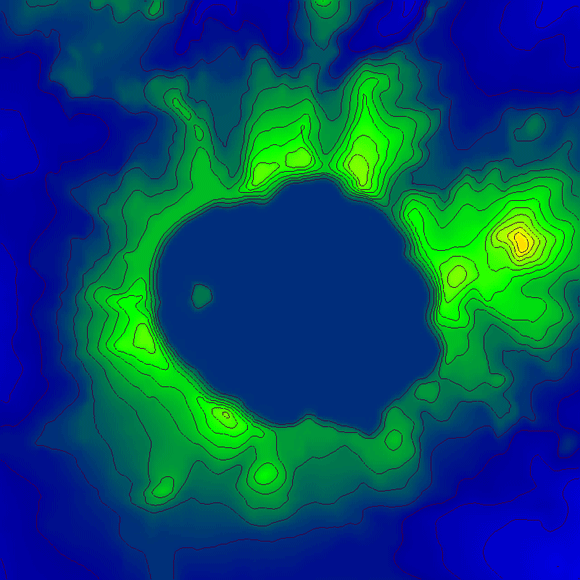
\includegraphics[width=0.5\textwidth]{imgs/226171_226171.png}
    \label{fig:isocontour-2d}
  }
  \subfloat[Three dimensional view of figure \ref{fig:isocontour-2d}]{
    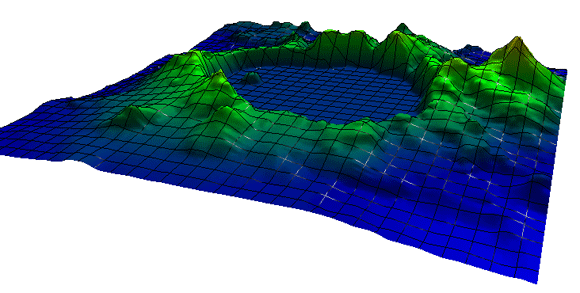
\includegraphics[width=0.5\textwidth]{imgs/226170_226170.png}
    \label{fig:isocontour-3d}
  }
\end{center}
\caption{Illustrations of heightmap, from: Intel Array Visualizer
  Gallery, \cit{intel}}
\label{fig:heightmap}
\end{figure}


For a level set representation there is an underlying function
describing the topology. Each contour corresponds to a set of points
in this function with the same value, thus we need a function which
produces a field of values. In heightmaps, it would be a function from
$(x,y)$ coordinates to a height. In general, any function producing a
field of values is sufficient.  

One function that has the desired characteristics is a function known
as the signed distance function $\phi$.

\section*{Outline of the report}

In chapter \vref{chap:sdf}, we give an in depth look on the signed
distance function, describe what kinds of mathematical operations we
have in our toolbox and describe the important reinitialize function in \vref{sec:reinitialize}.

Chapter \vref{chap:motion} deals with evolving the interface. In \vref{sec:extVel} we describe how to use an external velocity field, then in \vref{sec:intVel} we discuss using internally generated fields.

We have individually made a number of extensions to the basic level
set implementation. These extensions should show the versatility of
the method and show some practical applications.
In the final part of this paper, we look at these extensions. Each
section has been written by the person responsible for it.

First, in chapter \vref{sec:narrowband} Mikkel Vester presents a technique called "narrow band" which increases efficiency by limiting the area of calculations.
Then, Peter Kristensen talks in chapter \vref{sec:cuda} about his use of GPU multi-kernel programming to significantly improve performance.

The final two chapters present practical applications of level sets.
Martin Have has investigated and implemented a way of segmenting image data using level sets. He writes about his results in chapter \vref{sec:segmentation}.
In chapter \vref{sec:fluid} Sean Geggie presents how to use level set methods for evolving an interface to write a rudimentary simulator of incompressible fluids.



%%% Local Variables: 
%%% mode: latex 
%%% mode: auto-fill 
%%% TeX-PDF-mode: t 
%%% TeX-master: "../master.tex" 
%%% End:

